\subsection{Выбор алгоритмов}

Распределение будет происходить следующим образом:
\begin{enumerate}
    \item Вершины по очереди распределяются по хранилищам алгоритмом потокового распределения.
    \item При достижении некоторых значений размера вручную включается уточнение алгоритмом структурной оптимизации.
    \item По завершении добавления снова происходит уточнение алгоритмом структурной оптимизации.
    \item Выполнение запросов.
    \item Перераспределение вершин с учётом нагрузки (по ручному сигналу).
\end{enumerate}

Следовательно, для выполнения поставленной задачи нужно выбрать четыре метода:
\begin{itemize}
    \item Алгоритм потокового распределения.
    \item Алгоритм структурной оптимизации.
    \item Алгоритм структорной оптимизации с учётом нагрузки.
    \item Алгоритм поиска пути.
\end{itemize}

Для решения задачи потокового распределения, а также задания начального распределения был выбран алгоритм Fennel, описанный в разделе \ref{section:Fennel}. Основными причинами выбора Fennel являются низкая вычислительная сложность, возможность работы с крупномасштабными графами и поддержка балансировки партиций при минимизации числа разрезанных рёбер. Также он даёт наилучшее распределение из имеющихся методов потокового распределения, что важно для алгоритма уточнения

Для последующей структурной оптимизации распределения был выбран грианичный алгоритм уточнения Кернигана-Лина, описанный в разделах \ref{section:KL1} и \ref{section:KL2}. Данный алгоритм позволяет выполнять локальное улучшение качества разбиения путём итеративного перемещения вершин между партициями с целью уменьшения стоимости edge-cut. Преимуществом алгоритма является возможность интеграции пользовательской функции стоимости, учитывающей особенности рабочей нагрузки системы.

Для учёта рабочей нагрузки запросов была выбрана концепция, основанная на подходе Schism (раздел \ref{section:schism}). В реализуемой модели каждому ребру графа назначается запросный вес

\begin{equation*}
w_q(e),
\end{equation*}

который изначально принимает значение

\begin{equation*}
w_q(e)=1.
\end{equation*}

В процессе выполнения запросов и поиска путей в графе веса рёбер увеличиваются при каждом использовании ребра в найденном пути. Таким образом, рёбра, активно участвующие в обходах графа, получают более высокие веса и становятся более значимыми с точки зрения оптимизации размещения данных.

Алгоритм Кернигана-Лина использует данные веса при вычислении стоимости разбиения. В результате оптимизация направлена не столько на уменьшение размера разреза, сколько на уменьшение суммарного веса разреза, с чём данный алгоритм справляется особенно хорошо \cite{MetisOG}.

Для поиска кратчайшего пути в графе используется алгоритм A* \cite{AStar}. Выбор данного алгоритма обусловлен простотой его реализации, высокой распространённостью и отсутствием специальных требований к механизму поиска пути в рамках рассматриваемой системы. Алгоритм обеспечивает эффективный поиск маршрута за счёт использования эвристической оценки расстояния до целевой вершины, что позволяет сократить количество просматриваемых вершин по сравнению с алгоритмом Дейкстры. Так как алгоритм крайне известен его отдельного разбора в рамках данной работе не будет.


\subsection{Архитектура программы}

Архитектура программы должна имитировать архитектуру конечного решения: то есть состоять из отдельных хранилищ, соединённых шиной для общения, а также присоединённого к ним мастера, через которого происходит управление системой. Общая схема представлена на рисунке \ref{fig:basic_architecture}.

\begin{figure}[h]
    \centering
    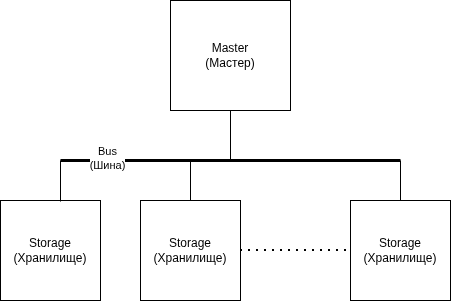
\includegraphics[width=0.6\textwidth]{extras/architeture.png}
    \caption{Общая схема архитектуры}
    \label{fig:basic_architecture}
\end{figure}

\subsection{Структуры данных}

Для реализации программы требуется реализовать следующие структуры данных:

\begin{itemize}
    \item Граф, включая:
    \begin{itemize}
        \item Ключ вершины.
        \item Вершина графа.
        \item Ребро графа. 
    \end{itemize}
    \item Хранилище (имитация).
    \item Шина (имитация).
\end{itemize}

Ниже представлены таблицы, описывающие эти структуры данных.

\begin{table}[H]
\centering
\begin{tabular}{|p{4cm}|p{4cm}|p{6cm}|}
\hline
\textbf{Поле} & \textbf{Тип} & \textbf{Описание} \\ 
\hline
key\_value & Шаблонный тип & Значение ключа вершины \\
\hline
\end{tabular}
\caption{Структура данных ключа вершины.}
\end{table}

\begin{table}[H]
\centering
\begin{tabular}{|p{4cm}|p{4cm}|p{6cm}|}
\hline
\textbf{Поле} & \textbf{Тип} & \textbf{Описание} \\ 
\hline
key & Ключ вершины & Ключ вершины \\ 
\hline
parameters & Индексируемый список произвольных данных & Набор произвольных параметров вершины \\ 
\hline
edges & Индексируемый список рёбер & Список смежных рёбер \\ 
\hline
\end{tabular}
\caption{Структура данных вершины}
\end{table}

\begin{table}[H]
\centering
\begin{tabular}{|p{4cm}|p{4cm}|p{6cm}|}
\hline
\textbf{Поле} & \textbf{Тип} & \textbf{Описание} \\ 
\hline
weight & Число & Запросынй вес ребра \\ 
\hline
directional & 1/0 & Признак ориентированности ребра \\ 
\hline
parameters & Индексируемый список произвольных данных & Набор произвольных параметров ребра \\ 
\hline
from & Ключ вершины & Начальная вершина \\ 
\hline
to & Ключ вершины & Конечная вершина \\
\hline
\end{tabular}
\caption{Структура данных ребра}
\end{table}

\subsection{Схемы алгоритмов}

\subsubsection{Fennel алгоритм}
Реализация Fennel алгоритма "вшивается" в хранилище, но часть действий происходит на мастере: Мастер отвечает за выбор хранилища для новой вершины, а каждое хранилище вычисляет локальную оценку размещения вершины.

\textbf{Работа мастера}

Работа алгоритма начинается с получения новой вершины вместе со списком её смежных рёбер. 
После этого мастер выполняет рассылку вершины всем хранилищам.

Каждое хранилище производит вычисление значения целевой функции и отправляет результат обратно мастеру. 
Мастер получает значения от всех хранилищ и выбирает хранилище с максимальным значением функции.

После выбора мастер рассылает уведомление о необходимости добавления вершины в выбранное хранилище.

\textbf{Работа хранилища}

После получения новой вершины хранилище начинает вычисление значения функции размещения.

Сначала вычисляется $p$ параметр хранилища, связанный с количеством вершин, уже находящихся в данном хранилище, нужный для балансировки. 
Затем выполняется проход по рёбрам вершины.

Для каждого соседа проверяется принадлежность текущему хранилищу. 
Если сосед уже размещён в данном хранилище, увеличивается счётчик локальных соседей

После завершения обхода рёбер вычисленное значение Fennel функции, которая использует $p$ параметр и счётчик соседей, отправляется мастеру.

\textbf{Добавление вершины}

После получения уведомления о размещении вершины хранилище проверяет, должна ли вершина быть добавлена локально.

Если вершина назначена данному хранилищу:
\begin{enumerate}
    \item вершина добавляется в хранилище;
    \item добавляются локальные соседи вершины;
    \item обновляются локальные связи.
\end{enumerate}

Если вершина назначена другому хранилищу, текущее хранилище сохраняет только внешние связи этой вершины для её соседей в этом хранилище.

После завершения операций обработка вершины считается завершённой.

\begin{figure}[H]
    \centering
    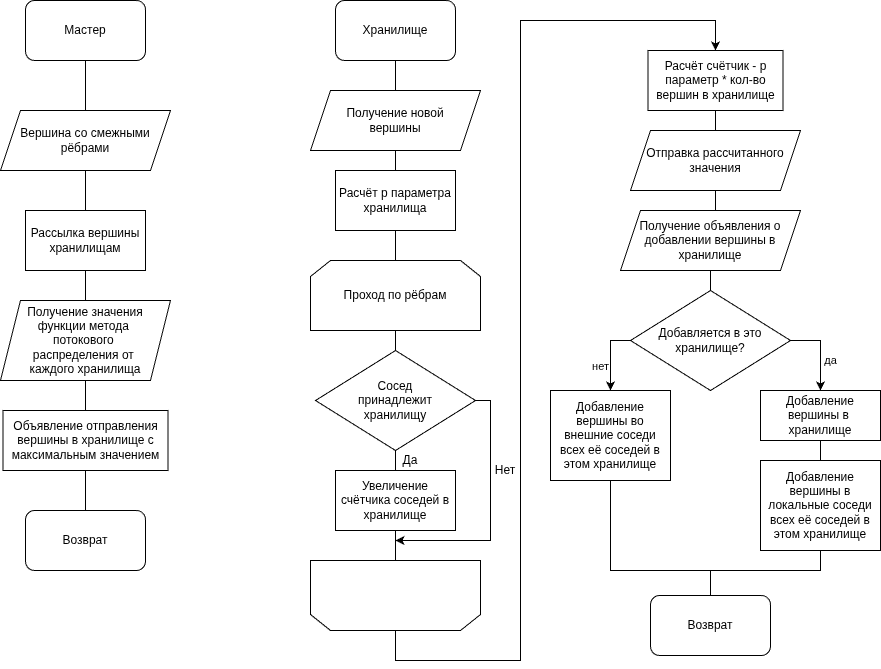
\includegraphics[width=\textwidth]{extras/contruction_part/Fennel.png}
    \caption{Схема распределения новой вершины в алгоритме Fennel}
\end{figure}

\subsubsection{Алгоритм Кернигана-Лина}

Реализация алгоритма Кернигана-Лина не вшивается в хранилище и является отдельным оптимизатором, работающим на мастере.

Алгоритм Кернигана--Лина используется для улучшения качества уже существующего разбиения графа между двумя хранилищами. 
Основная цель алгоритма заключается в уменьшении количества межхранилищных рёбер за счёт обмена вершинами между двумя хранилищами.

\textbf{Начало перебалансировки}

Перед началом выполнения алгоритма оба хранилища переводятся в режим перебалансировки. 
Для этого выполняется рассылка уведомлений о блокировке хранилищ, что предотвращает изменение структуры графа во время выполнения алгоритма.

После блокировки определяется множество граничных вершин. 
Граничными считаются вершины, имеющие связи с вершинами, расположенными в другом хранилище.

\textbf{Вычисление коэффициента перемещения}

Для каждой граничной вершины вычисляется значение $g_v$, характеризующее целесообразность её перемещения между хранилищами.

После вычисления значений начинается итерационный процесс перебалансировки. 


\textbf{Итерационный процесс}

Итерации продолжаются до тех пор, пока существуют вершины, которые могут быть перемещены, либо пока не будет достигнут лимит числа итераций.

Во время каждой итерации выполняется проход по всем граничным вершинам.
Для текущей вершины анализируется значение $g_v$:
\begin{enumerate}
    \item если значение положительно, вершина переносится в противоположное хранилище;
    \item после перемещения вершина помечается как уже обработанная;
    \item обновляется список граничных вершин;
    \item выполняется пересчёт значений $g_v$ для вершин, связанных с перемещённой вершиной.
\end{enumerate}

Если значение $g_v$ не является положительным, вершина остаётся в текущем хранилище.

\textbf{Обмен вершинами между хранилищами}

Так как алгоритм выполняется между двумя хранилищами, после принятия решения о перемещении вершины осуществляется обмен данными между узлами хранения.

Одно хранилище удаляет вершину из локального набора данных, а второе принимает вершину и добавляет её вместе с локальными связями. Так как обмен происходит объявлениями по шине, эти перемещения учитываются всеми хранилищами.
После завершения обмена обновляются сведения о принадлежности вершины и межхранилищных рёбрах.

\textbf{Завершение алгоритма}

После завершения всех итераций и отсутствия вершин, улучшающих текущее разбиение, алгоритм завершает работу.

Хранилища снимаются с режима блокировки и возвращаются в обычный режим обработки графа.

\begin{figure}[H]
    \centering
    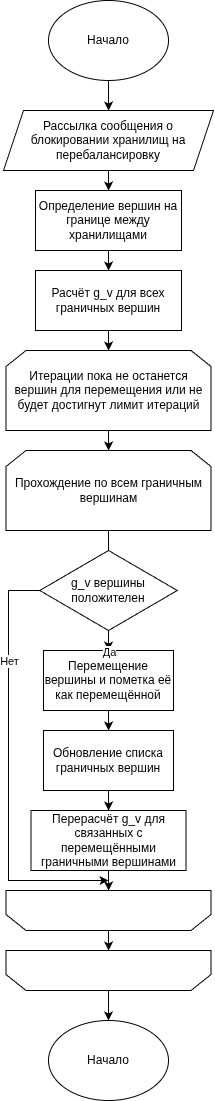
\includegraphics[height=0.8\textheight]{extras/contruction_part/KL.png}
    \caption{Схема уточнения распределения вершин алгоритмом Кернигана-Лина.}
\end{figure}